\documentclass[serif,mathserif]{beamer}
\usepackage{amsmath, amsfonts, epsfig, xspace}
%\usepackage{algorithm,algorithmic}
\usepackage{pstricks,pst-node}
\usepackage{multimedia}
\usepackage[normal,tight,center]{subfigure}
\setlength{\subfigcapskip}{-.5em}
\usepackage{beamerthemesplit}
\usetheme{chaosgroup}
\usepackage[utf8]{inputenc}
\usepackage[english,bulgarian]{babel}
\usepackage[T2B]{fontenc}
%4 people are authors - \author[Bruce Wayne]{Bruce Wayne \quad Clark Kent\\Peter Parker \quad Alan Scot}
\author[Йордан Маджунков]{Йордан Маджунков}


\title[Монте Карло\hspace{2em}\insertframenumber/\inserttotalframenumber]{Въведение в Монте Карло алгоритмите}

%\date{February 14, 2008} %leave out for today's date to be insterted

\institute{ 
\includegraphics[width=5cm]{chaoslogo_white.png}}

\begin{document}

\maketitle

% \section{Introduction}  % add these to see outline in slides

\begin{frame}
  \frametitle{Увод}
  Разни работи записани като точки\pause
  \begin{itemize}
  \item които изкачат\pause
  \item една \pause
  \item по една %leave out the \pause on the final item
  \end{itemize}
\end{frame}

% \section{Main Body} % add these to see outline in slides

\begin{frame}
  \frametitle{Математика}
  Писането на уравнения е лесно
  \begin{itemize}
  \item Просто ги копирайте от статията\pause
  \item или си ги напишете на ръка
    \begin{equation*}
      \textbf{p}^* = \underset{\textbf{p}}{\arg\!\min}~\sum_{\textbf{x}}\left[ I(\textbf{W}(\textbf{x};\textbf{p})) - T(\textbf{x}) \right]^2
    \end{equation*}
  \end{itemize}
\end{frame}

\begin{frame}
  \frametitle{Секси картинки}
  \begin{figure}[t]
    \centering
    \subfigure[материал 1]{
    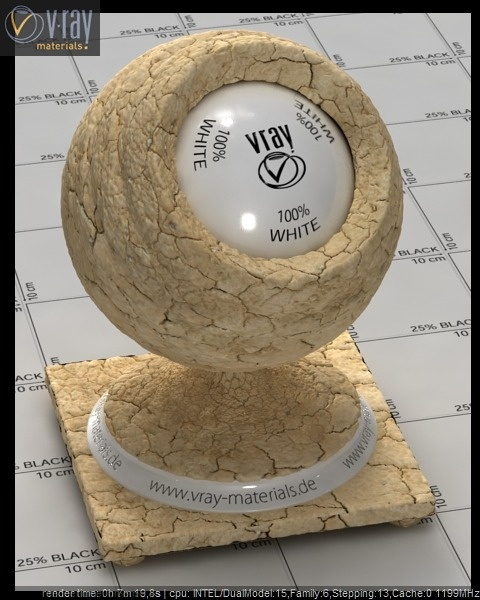
\includegraphics[width=3.2cm]{mat1.jpg}}
    \subfigure[друг материал]{
    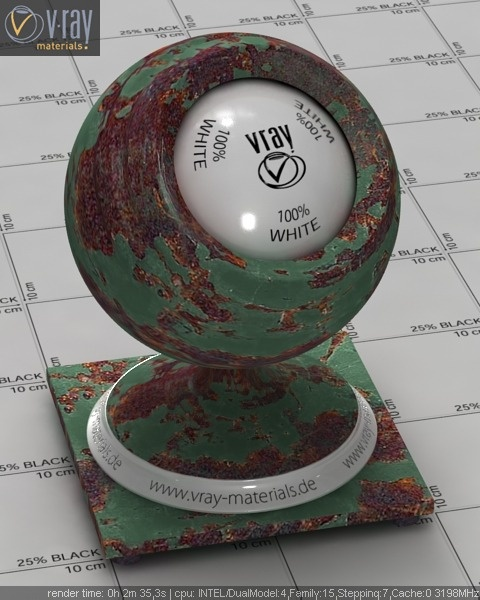
\includegraphics[width=3.2cm]{mat2.jpg}}
    \subfigure[още един]{
    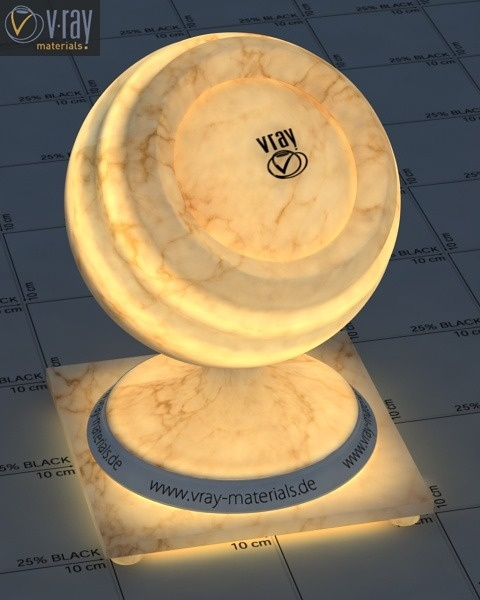
\includegraphics[width=3.2cm]{mat3.jpg}}
  \end{figure}
\end{frame}

\begin{frame}
  \frametitle{Филмче}
   Това не съм го пробвал дали работи.
  \begin{center}
    \movie[height=5cm,width=6.5cm,poster,autostart,loop]{}{leaves.avi}
  \end{center}
  \begin{itemize}
  \item Movies only seem to work in Adobe Reader
  \item Movie file is not embedded, it must be on the computer
  \end{itemize}
\end{frame}

% \section{Conclusion} % add these to see outline in slides

\begin{frame}
  \frametitle{Разни линкове}
  \begin{itemize}
  \item https://github.com/ymadzhunkov/cg2\_2015.git
%  \item Brought to you by www.shawnlankton.com
%  \item Please let me know about improvements!
%  \item This was supposed to look like a KeyNote Show
%  \item inspiration: http://www.ucl.ac.uk/~ucbpeal/latexposter.html
%  \item inspiration: http://newsgroups.derkeiler.com/... (in code)
        %http://newsgroups.derkeiler.com/Archive/Comp/comp.text.tex/2007-11/msg00299.html
  \end{itemize}
\end{frame}

\begin{frame}
  \frametitle{Въпроси}
\end{frame}
\end{document}
